%%%%%%%%%%%%%%%%%%%%%%%%%%%%%%%%%%%%%%%
%                                     %
%    Header Start                     %
%                                     %
%%%%%%%%%%%%%%%%%%%%%%%%%%%%%%%%%%%%%%%

% Din A 4 page with font size 12
%\documentclass[a4paper, twosides, 12pt]{article}
\documentclass[12pt,a4paper]{article}
\usepackage[english]{babel}
\usepackage[T1]{fontenc}
\usepackage[utf8]{inputenc}

%von niko
%\usepackage[margin=1.5in]{geometry}
%\usepackage{algorithmic}
%\usepackage{subcaption}
%\usepackage{lettrine}
%\usepackage[sc,osf]{mathpazo}
%\usepackage{booktabs}
% Es wird nicht eingerckt
\parindent=0mm

% arabic numbers for page numbering
\pagenumbering{roman}

% Definition der Ränder
\usepackage[paper=a4paper,left=30mm,right=30mm,top=25mm,bottom=25mm]{geometry}

% for declaring and using colors
\usepackage[table]{xcolor}
% define color values here
\definecolor{myblue}{rgb}{0.94, 0.97, 1.0}
\definecolor{Gray}{gray}{0.8}

% for apacite references
% \usepackage{apacite}
% \bibliographystyle{apacite}

% add references to Table of Contents
\usepackage[nottoc]{tocbibind}

% environment for definitions
\newtheorem{definition}{Definition}

\newtheorem{problem}[definition]{Problem}

% enumerate change
\usepackage{paralist}

% for romanic numbers
\newcommand{\RM}[1]{\MakeUppercase{\romannumeral #1{}}}

% for inserting graphics
\usepackage{graphicx}
\usepackage{subfigure}
\usepackage{tikz}
\usetikzlibrary{arrows,shapes,positioning,shadows,trees}
\tikzset{
  basic/.style  = {draw, text width=3cm, drop shadow, font=\sffamily, rectangle},
  root/.style   = {basic, rounded corners=2pt, thin, align=center,
                   fill=green!30},
  level 2/.style = {basic, rounded corners=6pt, thin,align=center, fill=green!60,
                   text width=8em},                                                  
  level 3/.style = {basic, thin, align=left, fill=blue!60, text width=6.9em}
}
\usepackage{wrapfig}

%\usepackage{pstricks}

% for inserting tables
\usepackage{tabularx, multirow, array, dcolumn}

% for mathematical symbols
\usepackage{amsmath}
\usepackage{amssymb}
\usepackage{latexsym}

% for graphics
\usepackage{tikz}
\usetikzlibrary{arrows,positioning}
\usepackage{color}

%for ipa
\usepackage{tipa}

% pdf LaTeX for linguistic examples
\usepackage{linguex}

%%for OT tables
\usepackage{pifont}    %for pointing hand
\usepackage{arydshln}    %for dashed lines
\usepackage{rotating}    %for angled text

% for inserting pdfs
\usepackage{pdfpages} 

% for inserting trees
\usepackage{qtree}
%\usepackage{ps-trees}

% for line distance
\usepackage{setspace}

% for thick lines
\usepackage{booktabs}

% for footer and header
\usepackage{fancyhdr}

%resizing
\usepackage{adjustbox}

% landscape format
\usepackage{lscape}
% for caption formatting
\usepackage{caption}

% for quotation marks
\newcommand{\Gu}{\glqq{}}		% quotation marks top
\newcommand{\Go}{\grqq\xspace} 	% quotation marks bottom
\newcommand{\Ga}{\textquotedblleft{}} % american quotation marks top start
\newcommand{\Ge}{\textquotedblright\xspace} % american quotation marks top end
\newcommand{\Tg}[1]{\textsubscript{#1}}		% lower
\newcommand{\Hg}[1]{\textsuperscript{#1}}	% higher
\newcommand{\leer}{\vspace*{\baselineskip}}% empty line

% reference with \tab, \fig, \sec to tables, graphics, and paragraphs
\usepackage{titleref}
\usepackage{prettyref}
\newrefformat{tab}{siehe Tab. \ref{#1} "\titleref{#1}" auf der Seite \pageref{#1}}% tables
\newrefformat{fig}{siehe Fig. \ref{#1} "\titleref{#1}" auf der Seite \pageref{#1}}% graphics
\newrefformat{sec}{siehe Abschnitt \ref{#1} "\titleref{#1}" auf der Seite \pageref{#1}}% paragraphs
%\pageref{#1}

%changes the numbering of figure and table
\numberwithin{figure}{section}
\numberwithin{table}{section}
\numberwithin{definition}{section}

% heading tweaks
\usepackage{titlesec}
\titleformat{\section}
{\normalfont\Large\bfseries}
{\thesection}
{1em}
{}
\titleformat{\subsection}
{\normalfont\Large\bfseries}
{\thesubsection}
{1em}
{}
\titleformat{\subsubsection}
{\normalfont\Large\bfseries}
{\thesubsubsection}
{1em}
{}

\newcommand{\HRule}{\rule{\linewidth}{0.5mm}}

% global scaling of table size
\usepackage{etoolbox}

\AtBeginEnvironment{tabular}{\scriptsize}
\AtBeginEnvironment{tabularx}{\scriptsize}

% Bibliography
\usepackage[style=authoryear,backend=biber]{biblatex}
\addbibresource{bibliography.bib}

%%%%%%%%%%%%%%%%%%%%%%%%%%%%%
%                           %
%      Document Start       %
%                           %
%%%%%%%%%%%%%%%%%%%%%%%%%%%%%
\begin{document}
\begin{titlepage}
\begin{center}

% Upper part of the page. The '~' is needed because \\
% only works if a paragraph has started.
%\\textsc{includegraphics[width=0.68\textwidth]{bilder/unilogo.png}~\\[1.5cm]
%~\\[1.5cm]
%\vspace{-1.0cm}}

\textsc{\LARGE Master's Thesis}\\[0.8cm]

\textsc{\large in Computational Linguistics}\\[0.5cm]

% Title
\HRule \\[0.4cm]
{  \bfseries \fontsize{22}{37} \selectfont Deconstructing Constructed Languages}\\
\vspace{0.4em}

\HRule \\[1.5cm]



% Author and supervisor
\begin{minipage}{0.4\textwidth}
\begin{flushleft} \large
\emph{Author:}\\
Connor \textsc{Kirberger}
\end{flushleft}
\end{minipage}
\begin{minipage}{0.5\textwidth}
\begin{flushright} \large
%\emph{1st Examiner \& Supervisor:} \\
\emph{Supervisors:} \\
Çağrı \textsc{Çöltekin} \\
Christian \textsc{Bentz}\\
\end{flushright}
\end{minipage}


\vfill



\textsc{\large Seminar f\"ur Sprachwissenschaft\\Eberhard-Karls-Universit\"at T\"ubingen}\\[1.5cm]



% Bottom of the page
{\large December 2023}

\end{center}
\end{titlepage}


%---------------------
% Ende der Titelseite
%---------------------

%----------------------------
% Selbstständigkeitserklrung
%----------------------------

\noindent

Hiermit versichere ich, dass ich die Arbeit selbständig verfasst, keine anderen als die angegebenen Hilfsmittel und Quellen benutzt, alle wörtlich oder sinngemäß aus anderen Werken übernommenen Aussagen als solche gekennzeichnet habe und dass die Arbeit weder vollständig noch in wesentlichen Teilen Gegenstand eines anderen Prüfungsverfahrens gewesen ist und dass die Arbeit weder vollständig noch in wesentlichen Teilen bereits veröffentlicht wurde sowie dass das in Dateiform eingereichte Exemplar mit den eingereichten gebundenen Exemplaren übereinstimmt.\\[4em]
I hereby declare that this paper is the result of my own independent scholarly work.
I have acknowledged all the other authors' ideas and referenced direct quotations
from their work (in the form of books, articles, essays, dissertations, and on the
internet). No material other than that listed has been used.
\\[18mm]
T\"ubingen, \today \hspace{6.0cm} \\%[10mm]\\
\begin{flushright}

\rule{0.4\textwidth}{0.2pt}\\
Firstname Surname
\end{flushright}
\pagestyle{empty}
\newpage

% inserting official anti-plagiarism statement
% \includepdf{antiplagiatserklaerung.pdf}
\newpage
%------------
% Textanfang
%------------

%% Inhaltsverzeichnis
\tableofcontents
\thispagestyle{empty}
%% Anderthalbzeiliger Zeilenabstand ab hier
\onehalfspacing
%\singlespacing

%% Keine Seitenzahl
\pagestyle{empty}

%% Beginn einer neuen Seite
\newpage

%% Abstract
\abstract{

Write the abstract here.
}
\newpage

%% Beginn einer neuen Seite
%\newpage

%%list of figures
\listoffigures
% list of tables
\listoftables


% list of abbreviations
\section*{List of Abbreviations}
\addcontentsline{toc}{section}{List of Abbreviations}

\begin{tabular}{lcl}
\textbf{API} & ~~~ & Application Programming Interface \\
\textbf{NLP} & ~~~ & Natural Language Processing \\
\textbf{PCA} & ~~~ & Principal Component Analysis \\
\textbf{TF-IDF} & ~~~ & Term Frequency - Inverse Document Frequency \\
\textbf{RNN} & ~~~ & Recurrent Neural Network \\
\textbf{LSTM} & ~~~ & Long Short-Term Memory \\
\textbf{SVM} & ~~~ & Support Vector Machine \\
\textbf{XML} & ~~~ & eXtensible Markup Language \\
\textbf{TTR} & ~~~ & Type-Token Ratio \\
\textbf{MATTR} & ~~~ & Moving-Average Type-Token Ratio \\
\textbf{IAL} & ~~~ & International Auxiliary Language \\
\textbf{SVO} & ~~~ & Subject-Verb-Object \\
\textbf{SOV} & ~~~ & Subject-Object-Verb \\
\textbf{IALA} & ~~~ & International Auxiliary Language Association \\
\textbf{LFN} & ~~~ & Lingua Franca Nova \\
\textbf{CSV} & ~~~ & Comma-Separated Values \\


\end{tabular}
\newpage

%\listoftables
%\newpage

%% header with section heading and right-aligned page number
\pagestyle{fancy}
\fancyhf{}
\fancyhead[L]{\textcolor{gray}{\slshape\nouppercase{\rightmark}}}
\fancyhead[R]{\thepage}
\fancyfoot[R]{\textcolor{gray}{Seminar für Sprachwissenschaft Universität Tübingen}}
\renewcommand{\headrulewidth}{0.4pt}

\renewcommand{\headrulewidth}{0.5pt}
\renewcommand{\footrulewidth}{0.5pt}



%--------
% TEXT
%--------
% page numbers start with 1 here.
\setcounter{page}{1}
\pagenumbering{arabic}

\section{Introduction \& Motivation} 
\label{sec:intro}

% Note the choice of "constructed language" in this paper as opposed to other terms, since there is debate, conflation, confusion, and difference in usage at times 

Constructed languages---also called artificial languages, invented languages, planned languages, engineering languages, glossopoeia, or more simply as "conlangs" \parencite{douglas2015book}---are languages that are consciously and purposefully created for some intended use, usually being defined in antithesis to the spontaneous and organic method in which natural languages arise and develop \parencite{sanders2016article}. These variations of the term are often, but not always, used interchangeably, as linguists do not all agree upon a core term due to personal preferences \parencite{Adelman2014article}, and there are sometimes differences in nuance depending on the context in which they appear. This thesis will mainly refer to them as constructed languages for simplicity.

The intended uses for which they are created can range broadly. Some are made specifically for fictional media, often seen in the genres of fantasy or science-fiction, with some more well-known examples being J. R. R. Tolkien's Elvish languages (e.g., Quenya, Sindarin, Nandorin) found in the world of Middle-earth in his writings, Marc Okrand's Klingon language from the Star Trek universe, and David J. Peter's Dothraki language used in George R. R. Martin's A Song of Ice and Fire novels along with their television adaptation, Game of Thrones \parencite{punske2020book}. Others are created to function as international auxiliary languages (IALs)---languages planned for the use of international and cross-cultural communication \parencite{Gobbo2016article}. The most well-known example (based on estimated number of speakers) of these is Esperanto, created in the 19\textsuperscript{th} Century by L. L. Zamenhof. Typically, constructed languages are distinguished and categorized based on these communicative functions. This will be discussed more comprehensively in section \ref{sec:background}. 

% Mention somewhat confusing cases, like "controlled" languages as another example of this blurred line between natural and artificial language or sign languages
% Consciously or subconsciously, conlangs' creators take inspiration and influences from already existing languages, be it natural or even other constructed languages \parencite{Oostendorp2019book}. 

Despite being defined in contrast to one another, however, constructed and natural languages are not necessarily opposite to one another characteristically. Aside from their origins, the boundaries between the two are not always clear when analyzed in greater detail \parencite{goodall2022article}. For example, \textcite{Schubert1989inbook} argues that some languages which are considered "natural" have some degree of artificiality, such as standardized written German and English differing from their spoken forms, and that the reverse is also true of some languages which are considered "artificial" because they draw from aspects of natural languages. As such, he believes human languages exist on a continuum of the two labels, rather than in the binary distinction---a view echoed by other linguists as well \parencite{Novikov2022article}. 

% Mention lack of existing studies specifically comparing/analyzing natural vs constructed languages using machine learning methods
% Expand more on Greenberg and Chomsky principles for linguistic universals, Universal Grammar, etc. and how it relates to this study (Mairal 2006)
% Schubert 1989 argued "no sharp distinction between ethnic and planned languages can be easily found, because any human language can be put in a continuum between naturalness and artificiality"
% Mention interest in deciphering old manuscripts, such as Voynich manuscript or Copiale Cipher, and how such a classification task could be useful in ruling out other possibilities and theories about the text's underlying language (one theory for example is that it's not a natural language)
% [DELETED] The former of the two proposed a framework for identifying the existence and extent of universals in languages based on empirical analysis of their surface structures (i.e. typology)

In many ways, the investigation into the disparity between the these two kinds of languages overlaps with the broader debate regarding what constitutes a language. Central to this debate is the search for linguistic universals---properties shared by all languages \parencite{Mairal2006book}. The concept of universals in language is recognized as one of the most important areas of research in linguistics \parencite{Christiansen2009book} and has served as a foundation for much linguistic theory, especially in more recent history, stemming largely from the influential theories and works of Greenberg \parencite{Greenberg1970book} and Chomsky \parencite{Chomsky1957book,Cook2007book}. 

Analyzing their surface structures can reveal whether or not constructed languages adhere to the same linguistic conventions as their natural counterparts. If machine learning models fail to successfully distinguish between the two, it may reinforce the notion that these universals are present in all languages, regardless of origin. Conversely, the models succeeding may suggest the opposite. In short, the primary motivation behind this thesis is to contribute to this ongoing debate through the application of machine learning, and a hope to learn more about the fascinating genre of constructed languages.

% Furthermore, while research on constructed languages is far from being novel, in the field of computational linguistics it is less common. Thus, my motivation here was to try something relatively new: to formulate this question of binary distinction based on linguistic features into a classification task and use machine learning methods to attempt to answer it.

\subsection{Scope of Study \& Research Question}
\label{ssec:scope}

% Make note of empirical differences between languages such as phonemes, word order, syntax, etc and explain how this study differs/specifies its focus
% [DELETED] As previously noted, the specific boundaries which separate constructed from natural languages are not always clearly or consistently defined---even amongst linguists.

The present work analyzes various linguistic features of both types of languages and seeks to make a comparison on the differences, if any exist, between them. More specifically, this study presents a binary classification task using decision tree and outlier detection models to determine if they can be distinguished from one another, based on the specific features examined and using a parallel dataset. 

Because of the wide-ranging nature of conducting such a broad analysis, there will of course be many features left unconsidered or excluded, intentionally or otherwise. With this in mind and following the precedent set by other related research on this topic, the main focus for features relate to entropy, morphological complexity, and overall lexical diversity.

The following is a breakdown of the structure of this thesis from here onward: the next section provides relevant background information, including an overview on constructed languages and a comprehensive review of related literature that examines the prior theoretical groundwork laid for exploring linguistic similarities and differences between constructed and natural languages; section \ref{sec:methodology} covers in detail the methodology taken in this research, from an explanation of the data used to the various experiments performed; section \ref{sec:results} presents the results of the study and discussion of these follows in section \ref{sec:discussion}; lastly, section \ref{sec:conclusion} consists of a conclusion as well as elaboration for possible future work.

\newpage
\section{Background}
\label{sec:background}

The vast landscape of linguistic research comprises a myriad of literature delving into the intricacies of languages, both natural and constructed. As this paper is concerned with constructed languages in particular and possible distinctive properties they may have, this section begins with a brief overview of their history and development, which provides some relevant context. Following this is an overview of some related literature, which is relevant to understanding the motivation behind the various computational approaches I employ in my experiments. 

\subsection{History of Constructed Languages}
\label{ssec:historyofconlangs}

% How much discussion here should overlap or be mutually exlcusive from the later section of me describing the data and languages used. Where would some of this information best fit? Or should I reorganize the sections? I feel I need to give a background on the history of constructed languages, since it's relevant here anyways and it includes a lot of information about the languages I'm using in particular. But then later during the data section of the methodology, I at one point thought to give brief descriptions of them there and introduce them. How should I organize and do this?
% Discuss the history of constructed languages, beginning with so-called philosophical languages of the 17th century (Goodall 2022)
% Discuss different theories of classifying/defining natural from constructed languages
% Other criterion for distinguishing types of constructed languages: a priori vs a posteriori dichotomy (Novikov 2022) and exoteric vs. esoteric dichotomy (Gobbo 2011) 
% Related quote: "The question is at what point we can call a constructed object a language. A useful taxonomy has been proposed by Blanke (1989), who envisaged a three-way distinction of ‘projects’, ‘semi-languages’ and ‘languages’, where ‘projects’ are basically objects which never grew out of the initial grammars and lexicons written by their constructors. They can grow into ‘semi-languages’ and eventually ‘languages’ if they start satisfying a whole list of criteria such as being used in written communication in books and journals, or having specialized vocabulary about a number of topics, etc. where languages are distinguished from semi-languages by having native speakers. According to Blanke, Esperanto is the only full ‘language’ in the set of constructed objects; as Blanke was a leading figure in the Esperanto movement" - Oostendorp
% Mention critique of eurocentrism surrounding constructed languages (the influences/inspirations they derive from), mentioned in Novikov 2022 page 9
% Related to above, Gobbo 2016 section 3 discusses international auxiliary languages including the sourcing of esperanto from western european languages (same for interlingua)
% Type of planned/constructed language makes a difference; Gobbo 2016 says "The ultimate goal of the planned language is important. Secret languages present different characteristics compared to IALs like Esperanto or Volapük: in order to preserve their secrecy, they often show morphological irregularities, in order not to be decrypted by the casual reader. As a consequence, secret languages do not necessarily show grammar reduction and morphological simplicity."
% Gobbo 2016 (page 39) mentions surface level differences in linguistic complexity between constructed and natural languages: " For ‘grammar reduction’, authors generally refer to the fact that planned languages show evident patterns of regularity in word formation, compared to natural languages, with few allomorphs, if any. For example, in English the plural of nouns is realized with various allomorphs (cat/cat-s, fox/fox-es, etc) while in Volapük, the first planned language with a community of supporters (see Section 4 below), there is only one form (vol/vol-s, pük/pük-s, ‘world/worlds’, ‘language/languages’), i.e. there is no allomorphy. Under the assumption that a language with less allomorphy is less complex, we conclude that Volapük is morphologically less complex than English."
% Important distinction when discussing planned languages: Gobbo 2016 writes "An important problem in such a comparison lies in the specificity of planned languages from a sociolinguistic point of view. Language architects can be traced in the development of many natural languages, such as Pompeu Fabra in the case of Modern Catalan (Costa Carreras, 2009), or Alessandro Manzoni in the case of Italian (Gensini, 1993). Pompeu Fabra and Alessandro Manzoni reshaped existing languages, which are alive thanks to a speech community that is actively involved in maintaining and promoting them. In other words, without a speech community, no language planning is possible. This process of reshaping is called ‘Ausbauization’ by Tosco (2011), from the classic term ‘Ausbau’ introduced by Kloss (1967)." In other words, the phrase 'language planning' can refer to actions taken for what are considered natural languages, too. Thus it is important to specify and distinguish this 
% On the origins of differentiating between purposes of constructed languages: Gobbo 2016 says "Alessandro Bausani (1974, 1970) was the first to notice that planned languages can be invented for different purposes."
% Don't forget to discuss Lingua Franca Nova too
% Okrent (2009) - "The history of invented languages is, for the most part, a history of failure."
% Mention sign languages, including Nicaraguan sign language
% italics for a prior and a posteriori?
% Contemporary conlangs are usually developed for one of three purposes: (i) to be an inter- national auxiliary language, known as an auxlang; (ii) to be a language used for an artistic endeavour, known as an artlang; or (iii) as a means of exploring certain philosophical concepts through constructing a language that embeds them, sometimes known as an engelang [2]. Constructed languages have also been categorized in terms of their method of creation. An a posteriori language is one that has been developed using aspects of other naturally occurring languages, while an a priori language is one that is created without intentional use of specific languages (Schreyer 2021)
% "planned languages are by definition based on the priority of writing over speech: they violate the priority of the spoken language over writing, one of the fundamental properties of natural languages, according to theoretical linguistics (Lyons, 1981, Section 4.2.1).2" (Gobbo 2017)
% "Despite the opportunities offered by the new technology, some of the online practices have been deemed questionable by the more scrupulous members of the conlang community: Google Translate offers Esperanto as one of its non-experimental languages, Wikipedia is available in eight different constructed languages (Esperanto, Volapuk, Ido, Interlingua, Kotava, Occidental, Lingua FrancaNova, Novial, Lojban) with Volapuk accounting for the largest number of articles (over 117,000, which places it 17th in the global rating, above the natural languages with millions of speakers), yet the overwhelming majority of them are the examples of low-quality machine translation." (Novikov 2022)

\textcite{okrent2009book} states, "The history of invented languages is, for the most part, a history of failure." She may be justified in saying this, depending on one's definition of failure in this context. From past to present, the total number of constructed languages may be as high as a thousand \parencite{Libert2016inbook,Schubert1989inbook,Schubert2001book}, with hundreds proposed for the purpose of being IALs in Europe alone \parencite{Schubert2001book}. Yet of these, only Esperanto is commonly considered to be successful in achieving its creator's intended goal of world-wide use as an auxiliary language (or rather that it is by far the most successful), with very few others even coming close, having a conservative estimation of two million speakers \parencite{okrent2009book}.

While the construction of languages is possibly as old as human history, they typically were not written down and were limited to in-group communication \parencite{Gobbo2016article}. The first documented endeavors came out of religious contexts and were likely used as secret languages, intentionally obscured and incomprehensible to lay people. In the 12\textsuperscript{th} century, abbess Hildegard of Bingen described and recorded a lexicon for Lingua Ignota, a Latin name meaning "unknown language". While extensive documentation of it (i.e., a grammar) was never found, it possessed a semiotic system based on Latin, German, and Greek. Later in the 14\textsuperscript{th} century, a group of Sufi mystics created Balaibalan, a language written in the Ottoman Turkish alphabet and which incorporated features of Persian, Turkish, and Arabic languages \parencite{Novikov2022article}.

Interest in creating such languages picked up in the 17\textsuperscript{th} century with the rise of so-called philosophical languages. In contrast to the last two, these languages were made to be more precise, less ambiguous, and better allow for philosophical reasoning (compared to natural language), such as by organizing world knowledge into hierarchies \parencite{goodall2022article}. Notable figures involved in making these include Francis Lodwick, Gottfried Leibniz, and John Wilkins, the latter of whose being arguably the most well-known and influential. Wilkins created a system of semantic categorization, cataloging all concepts in the universe \parencite{okrent2009book}, and then published his proposed language \parencite{Wilkins1968book}. An example of this hierarchal categorization can be seen in Figure \ref{fig:wilsonslanguageexample}.

% Include figure of Wilson's work or is it unnecessary? 

\begin{figure}
  \centering
        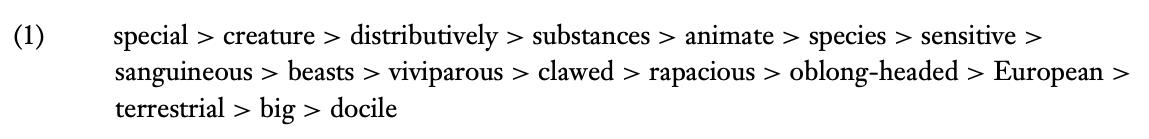
\includegraphics[width=1.0\textwidth]{WilsonsLanguageExample.png}
        \caption{Wilson's expression of "dog" in his philosophical language \parencite{goodall2022article}}
        \label{fig:wilsonslanguageexample}
\end{figure}

% It is from this category that the constructed languages used in the present study come from.
% Speak more about details of these IALs here? Or in the data section?

In the 19\textsuperscript{th} and 20\textsuperscript{th} centuries the focus for language construction, especially in Europe, shifted to that of making international auxiliary languages (IALs) intended to better enable communication across language barriers, i.e., people who do not share a similar language \parencite{goodall2022article}. Notably, this means they were generally designed to resemble natural language, with choice exceptions being the simplification of certain linguistic features. The surge in need for IALs correlated with the increase in prevalence and accessibility regarding international travel and communication at the time. Such languages were also described as "neutral" \parencite{Large1985book}, in the sense that individual advantages amongst speakers and learners would, theoretically, not exist due to IALs being second languages to everyone \parencite{Gobbo2016article}. That being said, many of the most prominent examples (e.g., Volapük, Interlingua, Esperanto, Ido) are derived from the Indo-European language family \parencite{Novikov2022article,goodall2022article}, so such a description might not be apt. A more detailed explanation of each of the IALs used in this study is provided in Section \ref{ssec:data}

% Discuss all of the IALs here? Or in the Data section instead? Or is it unnecessary to discuss them in such detail anyways?
% [DELETED] clubs were soon founded and spread around Europe and then to the United States and China, too \parencite{okrent2009book}. At its peak nearly a decade later, there were over two hundred societies and clubs, three hundred learning manuals \parencite{Gobbo2016article}, and twenty-five routinely published Volapük journals \parencite{okrent2009book}.
% (Gobbo 2008) for discussing Ido

% [DELETED] As the constructed languages examined and used in the dataset of the present work are all IALs, it would be beneficial to introduce them in more detail here. Volapük was made in 1879 by Catholic German priest Johann Martin Schleyer, who believed it was given to him by God. Argued to be the first successful constructed language due to amassing so many supporters \parencite{Gobbo2016article}, it soon died out in favor of Esperanto, which Ludwik Lejzer Zamenhof published in 1887.

% Mention other kinds of constructed languages, i.e. experimental or artistic ones like Solresol, Laadan, Lojban? (Adelman 2014)

Finally, there exist constructed languages that have been made for experimental, artistic, literary, or fictional purposes. In contrast to IALs, these languages are not made with the intention of replacing existing languages for everyday communication. Instead, their creators want to push the boundaries of language, test scientific hypotheses like linguistic relativity, or create a world, as is the case for the fictional examples provided in Section \ref{sec:intro}. Some other examples in this category include Solresol, a language that uses musical notes; Láadan, a language designed to be inherently feminist (i.e. more capable of expressing the female experience); and Loglan, a self-described "logical" language whose morphology and syntax are based on predicate logic \parencite{Adelman2014article}. Though it would be inaccurate to describe such languages as being only a recent invention, popularity in their conceptualization grew in the later part of the 20\textsuperscript{th} century.

While all share the defining characteristic of having been purposefully created, the linguistic features of constructed languages (e.g., phonetic, morphological, syntactical, lexical, orthographic) can vary immensely depending on factors such as, for example, their intended purpose for use or the other languages they draw from. An example of this was observed by \textcite{Gobbo2016article} in secret languages, specifically their tendency to have more complicated features, such as morphological irregularities, "in order to preserve their secrecy." Contrast to this are IALs, which have the opposite tendency for the sake of ease of communication and second-language acquisition, reflected in commonly assigned features such as SVO word orders, head-initial relative clauses, fronted \textit{wh-}phrases, and morphological regularity \parencite{goodall2022article,Gobbo2016article}. Section \ref{ssec:priorstudies} further examines research focused on linguistic features of these languages. 

In addition to this classification based on their intended communicative functions, i.e. as philosophical or international auxiliary languages, there are also taxonomies based on other criterion. For example, another frequently used distinction is that of \textit{a priori} and \textit{a posteriori} \parencite{Schreyer2021article,Gobbo2008article,Schubert1989inbook,Schubert2001book,Novikov2022article,Adelman2014article,Tonkin2015article}. Languages described as being \textit{a priori} are structurally entirely new \parencite{Tonkin2015article} and not based on existing languages, whereas so-called \textit{a posteriori} languages are the opposite, drawing from aspects of specific natural languages \parencite{Schreyer2021article}. \textcite{Gobbo2008article} also proposed the dichotomy of \textit{exoteric} (secret) and \textit{esoteric} (public) languages, derived from \textcite{Bausani1974book}. Similar to critiques regarding the distinction between constructed and natural, such dichotomies for categorizing constructed languages are also argued by some linguists to be more accurately described as scales instead, with many languages falling somewhere in the middle \parencite{Novikov2022article}. A final noteworthy classification scheme often cited by other linguists comes from \textcite{Blanke1989book} in the form of three classes: project, semi-planned, and planned. In short, these correspond to a set of steps that a constructed language must go through before it can be considered a "real" language \parencite{Schubert2001book}. 

A two-dimensional taxonomy for constructed languages containing several notables examples is shown in Figure \ref{fig:taxonomyplannedlanguages} \parencite{Gobbo2016article}.

% Include chart "taxonomy of planned languages" from Gobbo 2016 (fig 2). IMPORTANT QUESTION!!!!!! IS IT OKAY TO BORROW DIRECTLY LIKE THIS AS LONG AS I CITE IT?

\begin{figure}
  \centering
        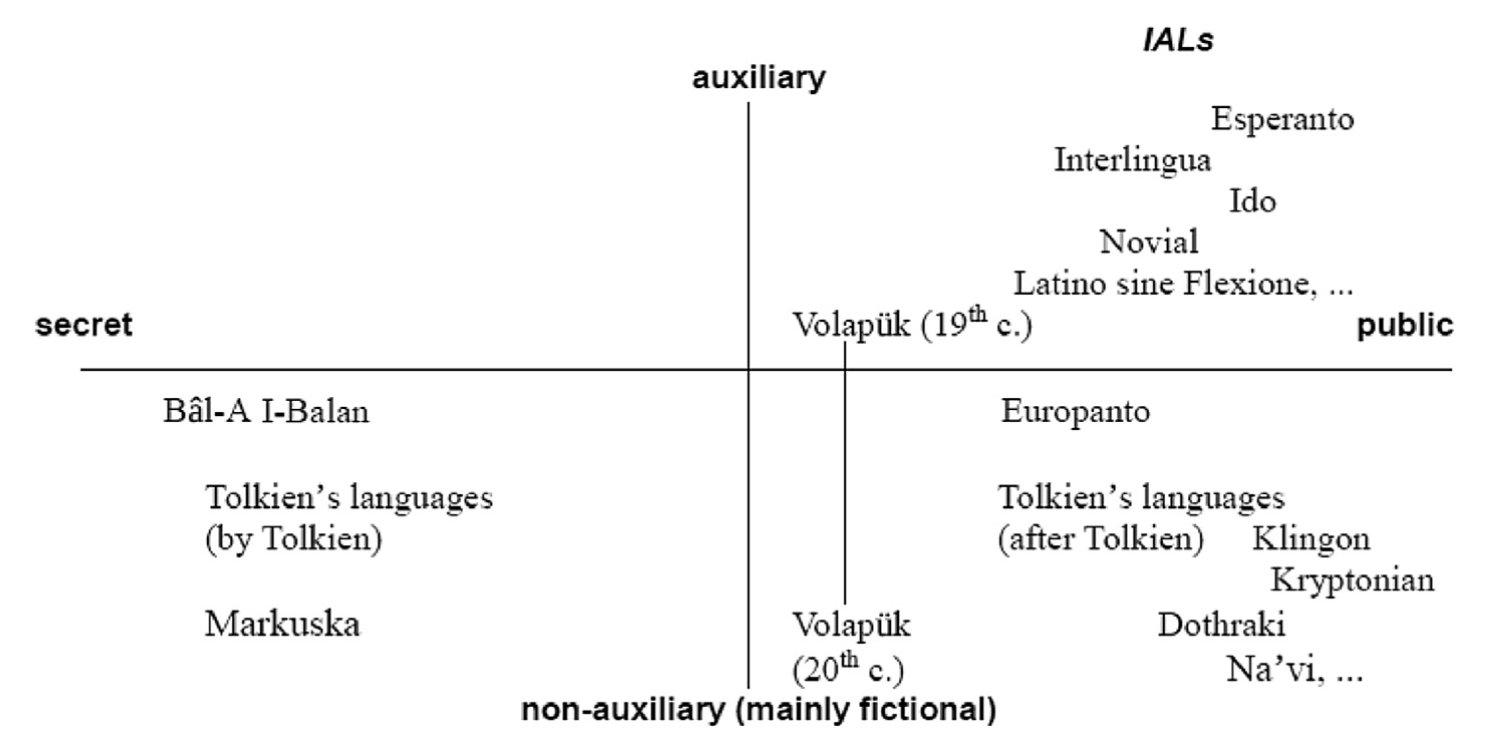
\includegraphics[width=1.0\textwidth]{TaxonomyOfPlannedLanguages.png}
        \caption{A taxonomy of constructed languages \parencite{Gobbo2016article}}
        \label{fig:taxonomyplannedlanguages}
\end{figure}

\subsection{Prior Studies}
\label{ssec:priorstudies}

% Prior studies comparing natural and constructed languages by linguistic features, prior studies on classification tasks for constructed languages

% Examining the Inductive Bias of Neural Language Models with Artificial Languages (White 2021)
% Are planned languages less complex than natural languages? (Gobbo 2016) 
% Constructed languages are processed by the same brain mechanisms as natural languages (Malik 2023)
% Constructive Linguistics for Computational Phraseology: the Esperanto Case (Gobbo 2019)
% On Pragmemes in Artificial Languages (Libert 2016)
% Authorship attribution, constructed languages, and the psycholinguistics of individual variation (Juola 2017)
% Sign language : a systematic review on classification and recognition (Sasidharan 2024)
% Morfessor-enriched features and multilingual training for canonical morphological segmentation (Rouhe 2022)
% How European is Esperanto? (Parkvall 2010)
% Complexity measurement of natural and artificial languages (Febres 2014)
% Native Esperanto as a test case for natural language (Lindstedt)
% Natural and Artificial International Languages: a Typosogist's Assessment (Comrie 1996)
% Evaluating the Irregularity of Natural Languages (Gomez 2017)
% From Esperanto to Volapük: A Graph-Based Approach to Assessing the Complexity of Constructed Languages (Sokolova)
% The word entropy of natural languages (Bentz 2016)
% Entropy of natural languages: Theory and experiment (Levitin 1994)
% Questions in Natural and Artificial Languages (Moskovsky)
% Morphology Matters: A Multilingual Language Modeling Analysis (Park 2021)
% Can Type-Token Ratio be Used to Show Morphological Complexity of Languages? (Kettunen 2014)
% Comparing comparatives in artificial languages
% What do complexity measures measure? Correlating and validating corpus-based measures of morphological complexity (Coltekin 2022)
% The effects of type and token frequency on word length: a cross-linguistic study (Berg 2022)
% Token-based typology and word order entropy: A study based on Universal Dependencies (Levshina 2019)
% Crosslinguistic Corpus Studies in Linguistic Typology (Schnell 2022)
% Data-driven Model Generalizability in Crosslinguistic Low-resource Morphological Segmentation (Liu 2022)
% The development of morphological complexity: A cross-linguistic study of L2 French and English (De Clercq 2016)
% Morpheme-Based Neural Machine Translation Models for Low-Resource Fusion Languages (Gezmu 2023)
% Bentz's papers
% Using the Relative Entropy of Linguistic Complexity to Assess L2 Language Proficiency Development (Sun 2021)
% Multiple studies on artificial language acquisition
% Prior studies on entropies of languages
% Prior cross-linguistic studies examining linguistic features like TTR of constructed/natural languages
% (Gobbo 2016) "The literature on planned languages is abundant and diverse, written in many languages and quite often outside of the usual peer-review system (Blanke, 2003), but in comparison to natural languages there are only few specific studies addressing the complexity of planned languages from the point of view of learnability. For instance, Jansen (2012) addresses the problems of learning the reflexive pronouns in Esperanto. In his review of the doctoral dissertation of Heil (1999), who compares the grammar reduction in French-based creoles and planned languages, Haitao (2001) rightly points out that more comparative work in this field is needed, and on a more solid basis."
% Performance of Robust Support Vector Machine Classification Model on Balanced, Imbalanced, and Outliers Datasets (Sembiring 2024)

In contrast to the abundance in literature and cross-linguistic analyses done on natural languages, similar research which also includes constructed languages is relatively sparse. In particular, while there is research that analyzes specific instances of linguistic differences between certain natural and constructed languages, large-scale cross-linguistic studies which utilize computational methods to classify the two based on linguistic features are practically nonexistent. Consequently, the present study is a somewhat novel approach. However, there is precedent for this research and the specific features examined, as well as computational approaches used, which this section will describe.

As noted in the previous section, the creation of IALs often involved the intentional simplification of particular linguistic features to facilitate language acquisition, for instance having more regularity in their morphological systems. Intuitively, then, one would assume this translates to measurable differences in various aspects of linguistic complexity when compared to natural languages, which often have irregularities as a result of their development and evolution. When comparing Volapük and English, \textcite{GObbo2016} concluded that

Much of the literature on constructed languages focuses on Esperanto specifically.

% Evaluating the irregularity of natural languages (Gomez 2017) approximates entropy of written texts and finds differences between language families, also compares their results to Esperanto
% Discuss research and the justification for using  one-class svm, decision tree, and randomforest for outlier detection/binary classification

\newpage
\section{Methodology}
\label{sec:methodology}

In this section, I introduce the dataset for this paper and discuss the steps taken for preprocessing it, followed by discussing in detail the features examined along with the different methods involved in extracting them from the data, and finally the classification approaches and models employed on the feature set. A brief description of the various APIs and libraries used is also included in \ref{ssec:librariesandapis}. 

Since this study involves many different experiments and elements being analyzed, I will begin by explaining an overview of what all was done. The number of possible features and measurements of linguistic complexity which could be analyzed in such a study is extensive to say the least; however, the scope of this thesis focuses mainly on empirical measurements relating to lexical diversity, morphological complexity, and entropy, along with some others measurements which are commonplace to calculating linguistic complexity, and thus seemed appropriate to also include. More specifically, the features investigated are average word length, average sentence length, type-token ratio (TTR) of morphemes, average number of segmentations in a word, average number of forms per lemma, lexical TTR and the related moving-average type-token ratio (MATTR), lexical entropy, text entropy, and character and word distribution entropies. Once the features' values were calculated for each language, the task became that of classification and anomaly detection with three machine learning models: a one-class support vector machine (SVM), random forest, and decision tree. Lastly, the methods for evaluating the performances of these models are discussed, as is the Principal Component Analysis (PCA) performed on the data.

\subsection{Data}
\label{ssec:data}

In total, twenty-four languages are analyzed in this study. Six of these are constructed languages: Esperanto, Ido, Interlingua, Lingua Franca Nova, Volapük, and Kotava. The remaining eighteen are natural: German, English, Spanish, Polish, Vietnamese, Indonesian, Turkish, Tagalog, Hungarian, French, Finnish, Italian, Dutch, Occitan, Danish, Swedish, Afrikaans, and Icelandic. 

For consistency, only languages which are written using the Latin alphabet (including the use of diacritics) were chosen. This is mainly because the constructed languages in the dataset all use Latin alphabets, so the selection of natural languages followed the same criteria. Moreover, it allows for more uniform cross-linguistic analysis of features which are sensitive (e.g. in the case of character entropy) to writing systems.

% Plot the languages + their language families to have some kind of visual comparison (table also works, include some data points for comparing each language i.e. number of speakers, word order (what do I do when it isn't clear due to having a more free word order, like for Esperanto, Finnish, etc?))
% Explain why I had to build my own corpus rather than using one that already exists. What limits are present as a result of having to build my own? 
% Discuss their language families, writing scripts (why not Japanese or Chinese?), and why those 6 constructed languages specifically
% Explain which natural language families the conlangs are based on, and surface level distinctions they may have
% von Oostendorp's Constructed Language and Linguistic Theory cites information about Ido (and Interlingua) around pages 7-8, how it is different from Esperanto
% Write more in-depth about Ido, Esperanto, Interlingua, Volapük, and Lingua Franca Nova. Who created them, how many estimated speakers, their purpose for being created, etc. etc.
% Write differences between Ido and Esperanto, using specific examples (for ex, from Goodall 2022), same for Interlingua. For example, a chart comparing words/grammar in all the languages, like on page 6.
% Mention how for some calculations done in this work, such as entropy, domain and corpus size are important and can cause results to vary
% Comrie 1996 also breaks down Esperanto with examples
% Lindsedt 2006 writes about considering Esperanto as a natural language and breaks down properties of it as well. Gobbo 2011 (section 4) breaks down further the specific languages Esperanto comes from
% Write about the Eurocentricism of the constructed languages used here (their inspirations/influences) and how that may affect the results
% Mention the drawbacks of relying on Wikipedia data, such as difference in authors, etc
% Why didn't include lojban? or Novial? (Available data for it is way smaller)
% Discuss number of symbols (i.e. letters in the alphabet) for each language too

\subsubsection{Constructed Languages in the Dataset}
\label{ssec:constructedlanguagesinthedataset}

% Refer to https://docs.verbix.com/Conlangs/ for more info of these

All of the constructed languages in the dataset are IALs and were chosen because of their availability in the Wikimedia dumps and having data which is comparable in size, allowing for their use as parallel texts. I will briefly introduce each of them in this section, explaining where they come from, some notable typological features they have, and how they compare to each other.

Esperanto, the most widely-spoken constructed language and considered by many to be the most successful \parencite{Gobbo2008article}, was created in 1887 by Polish ophthalmologist L. L. Zamenhof. Zamenhof’s goal was to create a neutral, easy-to-learn language that would facilitate international communication. Esperanto is a highly regular language, with consistent grammar and a simplified, phonetic spelling system. It draws its lexical roots and syntax primarily from Romance, Germanic, and Slavic languages \parencite{Gobbo2008article,Gobbo2011article}, making it recognizable and familiar to speakers of many European languages, while also intentionally being made to have a comparatively simpler grammar that avoids some complexities found in natural languages, such as irregular verbs or noun cases. It also has a strong global community with speakers around the world, an array of written literature, and even a number of native speakers who learn it from birth---a distinguishing trait which sets it apart from other constructed languages \parencite{goodall2022article}. As a result of its success, Esperanto also serves as a direct influence for many other constructed languages that have come after it, one being Ido. 

Ido is a reform of Esperanto that was proposed in 1907 by a group of linguists led by Louis Couturat, a French philosopher and mathematician, and in fact is an Esperanto word meaning "offspring" \parencite{Schubert2001book}. Its creators sought to address what they saw as imperfections in Esperanto, particularly those related to orthography and morphology. For instance, Ido avoids the use of the accusative case and reforms some Esperanto words to make them more universally recognizable. Overall, though, Ido still retains much of Esperanto’s vocabulary and basic structure, and the two are mutually intelligible to a large extend \parencite{goodall2022article,Schubert2001book}. Like most of the remaining constructed languages to be discussed in this section---with the exception of Volapük---Ido has small but a dedicated community of speakers and enthusiasts.

Interlingua was developed by the International Auxiliary Language Association (IALA) with the assistance of linguist Alexander Gode, officially being published in 1951. The idea behind Interlingua for it to most recognizable to the greatest number of people without requiring prior study \parencite{goodall2022article}, with most attention having been spent on its lexicon. The IALA's stated goal was to not so much create a new international language, but rather present a standardized international vocabulary \parencite{Large1985book} ("international" here basically referring to Western Europe). It is largely derived from and resembles Romance languages (with lesser influence from Greek and Germanic languages) \parencite{Schubert2001book}. In fact, this intentional resemblance extends even to morphological irregularities such as allomorphy, with other irregularities also being introduced to the language to make it appear more natural \parencite{goodall2022article}, a contrast to other IALs like Esperanto.

Volapük was created in 1879 by Johann Martin Schleyer, a German Catholic priest who believed the language had been given to him by God. It features highly agglutinative structure and regular, yet complex, morphology. While being derived mainly from English, German, and Latin, roots in Volapük differ significantly to the point of being unrecognizable to speakers of these languages \parencite{goodall2022article}. Despite being argued to be the first successful constructed language due to its rise in popularity, having amassed a large number of supporters worldwide along with the formation of clubs and societies \parencite{Gobbo2016article}, various issues regarding its complexity led to a rapid decline and eventual fall from usage in favor of Esperanto.

% The grammar of LFN avoids complex conjugations, gender distinctions, and irregular verbs.
% Refer to grammar of LFN book

Lingua Franca Nova, also abbreviated as LFN, is a relatively recent constructed language created by linguist C. George Boeree in 1998. Its lexicon is based mainly on Romance languages, specifically French, Italian, Portuguese, Spanish, and Catalan, while its grammar is based on Romance creole languages \parencite{Pawlas2020inbook}. In particular, inspiration came from the similarly-named Mediterranean Lingua Franca, a pidgin that developed for trade in the Mediterranean basin and was used from the 11\textsuperscript{th} to 18\textsuperscript{th} centuries, as well as from other creoles, such as Haitian Creole. It can be written in both Latin and Cyrillic scripts, though this dataset only contains the former. 

% Refer to https://medium.com/@ads.fbchandusuvvari/discovering-the-beauty-of-kotava-language-a-journey-to-multilingualism-9a7cb367a209
% Refer to https://www.kotava.org/en/en_staaveem.php for specifics about the grammar

The last constructed language used is Kotava. Created by Staren Fetcey in 1978, Kotava stands out in this dataset as being an attempt at creating a culturally neutral \textit{a priori} language, free from any biases or influences of existing languages and based on a philosophy of linguistic egalitarianism. This intentionally designed uniqueness manifests in several of its linguistic systems, from morphology to syntax. For example, though word order in Kotava is not imposed, the most frequently used one is OSV, which is exceedingly rare in natural language. Other unique features include a 4\textsuperscript{th} person plural, object complements being introduced by a transitive preposition, and a lack of declension. 

% For conlangs, how should I call the languages they are drawn from? "Language influences" or is there a better way to say it?

\begin{table}[h!]
  \centering
  \renewcommand{\arraystretch}{1.5}
  \begin{tabular} {|p{5cm}|p{5cm}|}
  \hline
  \textbf{Conlang} & \textbf{Source Languages/Families} \\
  \hline
  Esperanto & Romance, Germanic, Slavic \\
  \hline
  Interlingua & Romance \\
  \hline
  Lingua Franca Nova & Romance \\
  \hline
  Volapük & Germanic \\
  \hline
  Kotava & N/A \\
  \hline
  Ido & Romance, Germanic, Slavic \\
  \hline
  \end{tabular}
  \caption{Constructed languages used in the study, together with their main respective source languages from which they were designed.}
  \label{tbl:conlangs}
\end{table}

Finally, it is worth drawing attention to the fact that each of these languages were constructed mainly from various European languages, with the exception of Kotava. Consequently, this may influence the models performing classification and be visible in the results. This will be explored in greater detail later in Section \ref{sec:discussion}.

Table \ref{tbl:conlangs} shows the dataset's constructed languages together with the main source languages they draw from (with \textit{N/A} for Kotava meaning \textit{not applicable}). Note, however, that this is not an exhaustive list of all of their language influences.

% "and more niche" with how many speakers?
% Discuss LFN being inspired by Mediterranean Lingua Franca https://en.wikipedia.org/wiki/Mediterranean_Lingua_Franca
% Its inclusion in my dataset is primarily due to it being used on Wikipedia as an available source language, and thus also having a Wikimedia dump file.
% The final constructed language used in this study is Lingua Franca Nova, created by Dr. C. George Boeree. Compared to the others discussed so far, it is much more recent in its creation, having first appeared in 1998 online. As a result of being both newer and more niche, there is considerably less existing research related to it. 

% As this study is cross-linguistic in nature, it would naturally be ideal to use parallel text corpora, as this would enable more conclusive comparative and comprehensive analysis. However, finding already existing parallel corpora that also includes constructed languages, particularly less common ones, posed a bit of a challenge. 

% Include Blanke's (Schubert2001book) description of Esperanto as the only successful planned language

\subsubsection{Natural Languages in the Dataset}
\label{ssec:naturallanguagesinthedataset}

The natural languages included in this study represent a broad spectrum of linguistic diversity, comprising a variety of families, geographic regions, and typological features. Although this representation is not necessarily equal in distribution, it is meant to serve as a contrast to the constructed languages in the dataset, which lack a similar extent of variety due to overwhelmingly having the same source languages. However, rather than delving into the same level of details for each of the eighteen languages here as I did for the constructed ones, I will instead introduce them by focusing mostly on their collective significance and summarizing some of their relevant linguistic traits.

% Explain some notable characteristics of indo-european/germanic/romance languages (inflectional, agglutinative, etc.)

The language families represented are Austroasiatic, Austronesian, Turkic, Uralic, and Indo-European, with the latter being both the largest worldwide based on number of speakers and the most represented in the dataset (12 out of the 18 natural languages). While language families are defined through their collective sharing of linguistic features and common ancestors, they also contain some degrees of in-group variance as a result of evolution over time and are thus further divided into different subgroups accordingly. For the Indo-European languages in the dataset, English, German, Dutch, Afrikaans, Swedish, Icelandic, and Danish all belong to the Germanic branch. Likewise, Italian, Spanish, French, and Occitan are in the Romance languages, and Polish is Slavic.

Hungarian and Finnish are two of the most widely-spoken Uralic languages, so their inclusion provides a representative sample of their group.

The remaining languages were included in order to have more variety beyond only Europe. These are Tagalog and Indonesian (Austronesian), Vietnamese (Austroasiatic), and Turkish (Turkic). 

In terms of morphological typology, 

% Language family breakdown, make a pie chart for this
% German - indo-euro - germanic 
% english - indo-euro - germanic
% spanish - indo-euro - romance
% polish - indo-euro - slavic
% vietnamese - austroasiatic 
% indonesian - austronesian
% turkish - turkic
% tagalog - austronesian
% hungarian - uralic
% french - indo-euro - romance
% finnish - uralic
% italian - indo-euro - romance
% dutch - indo-euro - germanic
% occitan - indo-euro - romance
% danish - indo-euro - germanic
% swedish - indo-euro - germanic
% afrikaans - indo-euro - germanic
% icelandic - indo-euro - germanic

\subsubsection{Wikimedia}
\label{ssec:wikimedia}

% Mention genre/domain?
% Example link to one of the files used: https://dumps.wikimedia.org/novwiki/20240701/ then select novwiki-20240701-pages-articles-multistream.xml.bz2 1.4 MB
% Mention the year/date of the file to specify the dump
% Which languages' files did you limit (using the max_articles variable) with the script? The biggest files (eo, da, fi, tr, id, vi, hu, sv, nl, pl, it, es, fr, de, en) I gradually limited the max number of files to be extracted from the dumps; max 50000 for eo, 

The data for this thesis comes from Wikimedia dump files. Wikimedia is a global movement and community founded on shared values, whose goal is to provide free and openly accessible information to everyone in the form of massive collaborative projects (which include, among others, the widely-used Wikipedia and Wiktionary). For a large, cross-linguistic study, massive databases with open-access make for an ideal source for corpora. Most importantly, the projects are multilingual, meaning data is available in a considerable number of different languages---including several constructed ones. This allows for composing a set of corpora which is adequately parallel to each other and from the same domain. Additional constructed languages which are also available from the dumps---but were not included in the present study due to having a much smaller amount of data---are Novial, Interlingue, and Lojban.

The dump files provide detailed, archived snapshots of the content from Wiki repositories for a specified point in time and are available in different formats. All dumps used were XML-formatted and from the 2024-07-01 archive, containing articles together with their metadata\footnote{\url{https://dumps.wikimedia.org/backup-index.html}}. It is also worth mentioning here that there are some drawbacks to using these dumps for the present study. The files sizes vary considerably depending on the language, with the largest being roughly 22 gigabytes (English) and the smallest around 4 megabytes (Lingua Franca Nova), meaning all files do not contain the exact same articles. Additionally, the open and collaborative nature of Wikimedia means the articles are often authored by a multitude of different people, which can result in inconsistencies in the texts, such as with writing style. Similarly, it may also produce an imbalance in the amount of information provided across languages, with the same article in one language being considerably more detailed than in another, and inconsistent or low-quality translations, as \textcite{Novikov2022article} noted to be the case for Wikipedia articles in Volapük. Thus, while Wikimedia was decided as the best available option for the task at hand, there are some unfavorable aspects of using it which may influence the results; this will be discussed more in Section \ref{sec:discussion}.

% Genre/domain of texts? Do all dumps have the exact same articles? How does this affect the experiment and results?
% Not gold standard corpus, its quality depends on many different variables (i.e. the wikipedia contributors who wrote the articles)
% Give a breakdown of the corpora data, for example the number of words/sentences for each language

\subsection{Data Preprocessing}
\label{ssec:datapreprocessing}

Preprocessing text data is essential for natural language processing (NLP) tasks, and since I essentially had to compile my own corpora for this study, meticulous effort was made to thoroughly clean all of the texts and obtain as close to a set of parallel data as possible.

% Preprocessed by excluding characters not in a language's alphabet, to attempt to account for words in foreign languages being used in the text data, however this has drawbacks in that it also excludes loanwords or proper nouns at times too. Additionally, I removed only the individual characters themselves, is it better (or possible?) to remove the entire word that they are part of instead? Or does it not make a difference? For example, in Kotava there is no letter 'h', the proper noun 'hiroshima' therefore would become 'irosima' with my method. 
% Explain more in depth the regex used and why. For example, I removed parantheses along with everything inside of them to try to maintain grammatical sentences without redundancy or fragments in the middle
% Removed subtitles of Wikipedia pages (by adding extra forward slashes '/////' in the WikiExtractor code, so it would be easily identified using Regex later)
% Wanted to keep full sentences (why? what's useful about having the texts as one sentence per line for your study? A: For entropy calculations, it makes sense to separate the data by sentence + line because if the sentences blur together it will change this value of entropy. Also consider sentence length), so there is not exact same word counts/sentence counts for all files. Include chart of total words/sentences for each language file?
% Mention why the WikiExtractor script was used in the first place
% Ex: python WikiExtractor.py --infn ~/Downloads/enwiki-20240701-pages-articles-multistream.xml.bz2
% Show some examples of the regex used from your code
% Show examples of before and after the preprocessing + show an example of the final preprocessed data

Text data was first extracted from the Wikimedia XML-formatted dump files with the use of WikiExtractor\footnote{GitHub repository for WikiExtractor: \url{https://github.com/attardi/wikiextractor}}, a Python script \parencite{Attardi2015wikiextractor} that I adapted by adding a limit to the number of articles in order to make extraction of the largest of the files (English in particular) less demanding and quicker. The output is a simple text file, which is a much easier format to clean and work with. 

I then used several regular expressions to remove general, unnecessary text from each file such as page titles, section headers, links, fragments, HTML tags, braces, and all other non-alphabet symbols aside from periods. This also includes the removal of parantheses and their contents. The text was then made all lowercase and split by the periods---while also attempting to account for abbreviations---to make separate sentences. This was done mainly to enable more accurate measurement of entropy later.

Following this, foreign symbols (i.e., characters not part of a particular language's alphabet) were removed for each text/language, as occasionally proper nouns, loanwords, etc. would appear in the text, which would also affect measurements of entropy, in addition to morphological segmentation and analysis. To give an example of this, there is no letter 'h' in Kotava, but this would sometimes be used in proper nouns such as 'Hiroshima'. After the text is cleaned, the remaining word left behind is 'irosima'. 

Finally, each text file was truncated according to the file size of the smallest corpus, LFN, so as to have similar lengths. This was calculated based on number of words, with the limit being 630000 (since this is roughly the number of words remaining in the LFN text file after cleaning), and while preserving complete sentences. Sentences containing only one word were also removed. The end result of pre-processing was a single text file corresponding to each language, with each line in the file being a single sentence. The corpora with the smallest and largest number of words is Kotava and Danish/Volapük at 617400 and 629999 words, respectively. For number of sentences, the smallest and largest corpora are Vietnamese and Volapük at 21115 and 55920 sentences, respectively. For a breakdown of these size for each language's text after pre-processing, refer to Table \ref{tbl:preprocessedtexts}.

\subsection{Libraries and APIs}
\label{ssec:librariesandapis}

Several libraries and APIs were used in both the feature extraction and classification parts of the study, and the most important of these will be briefly introduced here. In the field of machine learning, two of the most popular model frameworks used are \textsc{PyTorch} and \textsc{TensorFlow}, which are interacted with via the \textsc{torch} and \textsc{Keras} APIs, respectively. Aside from some relatively minor differences (e.g., the syntax of their code and performance optimization), they share a lot of similarities and are typically used according to personal preference. In the context of this paper, these frameworks are used for calculating some of the entropy values from the corpora. In addition to libraries used for constructing the model architectures, there are also ones used for the data itself. Arguably the most fundamental for this is \textsc{NumPy}, which stands for Numerical Python and is used to accomplish extremely fast and efficient computation of arrays. Other essential libraries include \textsc{Pandas}, used for data manipulation and analysis, and \textsc{Matplotlib}, used for visualizing data and plotting model results. Lastly, \textsc{scikit-learn} provides a wide range of tools for machine learning algorithms, data preprocessing, and model evaluation---as well as computation, thanks to it being built on top of \textsc{NumPy}. The models I used for classification (i.e., One-Class SVM, Random Forest, Decision Tree) as well as PCA come from this library. Altogether, these libraries are often used in tandem due to integrating so well with one another. 

\subsection{Feature Extraction}
\label{ssec:featureextraction}

% Briefly explain what feature extraction is and why I use it in this study (?)
% Come back to edit later:
% Once the data had been preprocessed, some initial values were calculated to be used as a starting point for our investigation in comparing natural and constructed languages. These were Zipf's law of abbreviation, type-token ratio (TTR), moving-average type-token ratio (MATTR), and character and word distribution entropies.
% Refer to https://medium.com/analytics-vidhya/feature-extraction-techniques-pca-lda-and-t-sne-df0459c723aa

% Mention in each subsubsection why the particular feature was extracted, why it was seen as a possible indicator or useful information in this experiment
% Mention use of StandardScaler(), etc.
% torchrnn.py is for text entropy, kerasrnn.py and reversekerasrnn.py are for lexical entropy
% Also include calculations like average sentence length, average word length!!!

A crucial step in many NLP tasks is feature extraction. Before training the classifiers for anomaly detection, 

\subsubsection{Lexical Diversity}
\label{ssec:lexicaldiversity}

A popular way of measuring lexical diversity is with TTR, given by the formula \[TTR = \frac{\sum_{i=1}^{n}\delta(w_i)}{n}\]

where $\delta$ corresponds to 

A glaring issue with TTR, however, is that it can vary widely based on a text's length. The longer a particular text, the higher the likelihood of repetition occurring. There have been several solutions proposed to address this issue, one being MATTR. MATTR is given in the formula \[MATTR_i = \frac{TTR_1+TTR_2+...+TTR_i}{i}\]

\subsubsection{Morphological Complexity}
\label{ssec:morphologicalcomplexity}

% Mention the root languages the conlangs are based on (i.e. Esperanto and German) to explain/describe some of the morphological complexity of said conlang
% "A popular algorithmic way to approximate the morphological complexity of a language has been Patrick Juola’s (1998, 2008) suggestion of distorting word structures by using a unique random number for each different word type. After distortion, the data is compressed using a compression algorithm. Then the size of the compressed original word file is divided by the size of the compressed distorted word data file. The result tells the complexity of each language’s morphology on the basis of Kolmogorov complexity that the compression algorithm approximates." (Kettunen 2014)
% Show examples of the segmentations done by Morfessor
% Show examples/results of checking the accuracy of Morfessor's segmentations
% Using trained Morfessor model (for example, first training it on English corpus) to test its segmentation accuracy for other languages?
% Unsupervised morpheme segmentation and morphology induction from text corpora using Morfessor 1.0 (Creutz 2004)
% Morfessor EM+Prune: Improved Subword Segmentation with Expectation Maximization and Pruning (Gronroos 2020)
% Show example of morphological segmentation at beginning of this section (e.g. Gronroos 2020)
% Morfessor and hutmegs: Unsupervised morpheme segmentation for highly-inflecting and compounding languages (Creutz 2005 article2)
% Towards an unsupervised morphological segmenter for isiXhosa (Mzamo 2019)
% UNSUPERVISED SEGMENTATION OF WORDS INTO MORPHEMES ()
% Explain the morphological systems of the languages (e.g. agglutinative), include a table 
% (Mzamo 2019) "Minimum Description Length (MDL) [20] has seen extensive use in unsupervised morphological segmentation, primarily as a measure of fit of the training data to heuristic models and statistical models [21], [22]. The comparative standard used in this study, Morfessor-Baseline [23], uses MDL and Maximum likelihood estimation."
% Modeling Morphological Typology for Unsupervised Learning of Language Morphology (Xu 2020)
% Unsupervised Learning of Language Morphology by Exploring Language Typology (Xu)
% Morpheme-Based Neural Machine Translation Models for Low-Resource Fusion Languages (Gezmu 2023)
% Include Morfessor model's types/tokens from compounds in training data and number of epochs, and cost at each epoch and final cost and training time; e.g. for Esperanto: Compounds in training data: 67460 types / 67460 tokens, 7 epochs, Final cost: 1460075.939887648, training time: 227.798s
% Morfessor also run on remote server, and writes a training log
% For analysis (for each language): calculate type/token ratio of morphemes (number of unique tokens/morphemes over the total number of tokens/morphemes), average number of segmentations, average number of forms for each lemma
% When identifying the lemmas for each segment, using the largest segment. For cases of multiple largest segments, some options: frequency-based disambiguation (the segment which appears most often in the whole data is the lemma, etc) or take the first one (greedy algorithm) or take both/all of the equally largest as lemmas
% Refer to morfessor docs on Python library interface https://github.com/aalto-speech/morfessor/blob/master/docs/source/libinterface.rst

The morphological systems of each language were analyzed using \textsc{Morfessor 2.0}.  

% \subsubsection{Zipfian Distribution}

% Zipfian distribution of natural languages vs constructed languages, refer to Bentz 2023
% Zipf’s word frequency law in natural language: A critical review and future directions (Piantadosi 2014)

% Created word lists from the corpora
% Used Morfessor with logarithmic function
% Calculated morpheme TTR, etc.

After the text files were segmented, 

\subsubsection{Entropy}
\label{ssec:entropy}

In information science, entropy means... 

% Evaluating the Irregularity of Natural Languages (Gomez 2017) has more info for this section, starting on page 2
% Calculated character, word, text, and lexical entropies (and reverse)
% Describe the RNNs used for calculating these, as well as the server it was run on. Did not train on GPU!
% Mention suprisal
% Refer to https://www.cs.bu.edu/fac/snyder/cs505/PerplexityPosts.pdf for explanaion on perplexity
% Lexical Richness and Text Length: An Entropy-based Perspective (Shi 2020)

The entropy was calculated for the character and word distributions in each of the corpora, given by the following formula: \[H = -\sum_{i=1}^{n}p_{i}\log_{2}p_{i}\]

% Perplexity is related to entropy...
% Cross-entropy as the loss function...

% Text entropy calculated using Character-Level LSTM in PyTorch (torchrnn.ipynb) https://github.com/LeanManager/NLP-PyTorch/blob/master/Character-Level%20LSTM%20with%20PyTorch.ipynb (Use a footnote to cite)

% Lexical entropy (and reverse lexical entropy) calculated using Character-Level RNN in Tensorflow (kerasrnn.ipynb) 
% Explain about inverse lexical entropy, why it was calculated and what usefulness it may have? For example, if a language is very prefix-heavy vs. suffix-heavy, it may change the predictability of the characters of a word in the opposite direction
% the entropy value was taken from the val_loss of the model
% early stopping was used in the tensorflow models for lexical entropy, based on val_loss and with patience=3

For text entropy, a character-level long short-term memory (LSTM) model built with \textsc{PyTorch} was used.\footnote{Model adapted from \url{https://github.com/LeanManager/NLP-PyTorch/blob/master/Character-Level\%20LSTM\%20with\%20PyTorch.ipynb}}

\subsubsection{PCA}
\label{ssec:pca}

% "To analyze whether measures include multiple dimensions or not, we perform dimensionality reduction using principal component analysis (PCA). The intuition here is that if the measures differ in what they measure, the explained variance should be shared among multiple principal components. Furthermore, if the lower-order principal components measure meaningful dimensions of morphological complexity, we expect them to indicate linguistically relevant differences between languages." (Coltekin 2022)
% Explain why you chose n_components = 0.95 for the PCA
% Use scree plot? Kaiser's rule?
% Do a breakdown of how PCA and explained variance (the mathematics) works, following https://machinelearningmastery.com/principal-component-analysis-for-visualization/
% Do PCA in 2 or 3 dimensions/components? (for 3, refer to https://machinelearningmastery.com/principal-component-analysis-for-visualization/)

PCA is an unsupervised method of dimensionality reduction, used for  

% Discuss explained variance ratio
% Use https://www.jcchouinard.com/pca-explained-variance/ for visualizing explained variance

\subsection{Classification}
\label{ssec:classification}

% Visualizing the features (in a graph) prior to classification to analyze whether a linear or nonlinear model is required and why 
% Include tables of the hyperparameters for both models, explained how they were tuned (grid search, etc.)


\subsubsection{Decision Tree}
\label{ssec:decisiontree}

% Discuss pre-pruning the decision tree

Decision Tree Classifier...

\subsubsection{Random Forest}
\label{ssec:randomforest}

% Refer to https://towardsdatascience.com/a-practical-guide-to-implementing-a-random-forest-classifier-in-python-979988d8a263
% Refer to https://www.geeksforgeeks.org/random-forest-classifier-using-scikit-learn/
% Include visualization of finetuning, as shown by https://medium.com/@Doug-Creates/tuning-random-forest-parameters-with-scikit-learn-b53cbc602cd0

\subsubsection{One-Class SVM}
\label{ssec:oneclasssvm}

% Refer to https://www.analyticsvidhya.com/blog/2024/03/one-class-svm-for-anomaly-detection/ for "One-class SVM aims to discover a hyperplane with maximum margin within the feature space by separating the mapped data from the origin. On a dataset Dn = {x1, . . . , xn} with xi ∈ X (xi is a feature) and n dimensions:"
% Refer to https://www.analyticsvidhya.com/blog/2024/03/one-class-svm-for-anomaly-detection/ also for visualization of One Class SVM model performance
% Would it make sense to do this two times with the same model, once with the inlier class as conlangs and once as natlangs?
% Outlier detection and novelty detection
% Include mathematical equation for normalization/standardization/min-max scaling (refer to https://www.geeksforgeeks.org/how-to-normalize-data-using-scikit-learn-in-python/ or )
% Support Vector Method for Novelty Detection (Olkopf 2000)
% For adaptive OCSVM, refer to https://www.researchgate.net/publication/300242572_An_Adaptive_Weighted_One-Class_SVM_for_Robust_Outlier_Detection

One-Class SVMs are a special kind of SVMs used in the domain of anomaly detection. While similar to one another, classic SVMs separate two classes using a hyperplane with the largest possible margin. In contrast to this, One-Class SVMs...Rather than training on an entire dataset containing two classes as with classic SVMs, these models train exclusively on the majority class, also called the "normal" class. After training,  

Standardization is given by the formula \[X^{\prime} = \frac{X - \mu}{\sigma}\] 

where $\mu$ is mean and $\sigma$ is the standard deviation.

\subsection{Evaluation of Classifiers}
\label{ssec:evaluationofclassifiers}

% Methods for evaluating the accuracy, etc. of the classifiers, RNNs used for calculating the entropies (?), and morphological segementations with Morfessor (?)
% Should I use sklearn.metrics 'classification_report'? As done by https://medium.com/analytics-vidhya/feature-extraction-techniques-pca-lda-and-t-sne-df0459c723aa
% Use of Leave One Out Cross Validation for supervised methods (refer to https://www.statology.org/leave-one-out-cross-validation/), include MSE/MAE/Bernoulli likelihood formulas, etc

\newpage
\section{Results}
\label{sec:results}

This section reports the results of each of the methods implemented.
% Also do 1D analysis of all languages for each single dimension (e.g. the TTR, seeing if there's clustering or dispersal in tendency for the languages on a single line)

\subsection{Results of Lexical Diversity}
\label{ssec:lexicaldiversityresults}

% Include table showing number of tokens and types for each language, together with the ratio calculation

\subsection{Results of Morphological Segmentation}
\label{ssec:morphologicalsegmentationresults}

\subsection{Results of Feature Extraction}
\label{ssec:featureextractionresults}

\begin{sidewaystable}[h!]
  \centering
  \renewcommand{\arraystretch}{1.0}
  % \begin{tabular} {|m{1cm}|m{1cm}|m{1cm}|m{1.2cm}|m{1cm}|m{1.2cm}|m{1cm}|m{1cm}|m{1cm}|m{1cm}|m{1cm}|}
      % \centering
      \begin{tabular}{|c|c|c|c|c|c|c|c|c|c|c|c|c|c|}
      \hline
          \textbf{Corpus} & \textbf{Type} & \textbf{Avg Word Length} & \textbf{Avg Sentence Length} & \textbf{TTR} & \textbf{MATTR} & \textbf{Morpheme TTR} & \textbf{Avg Segs Per Word} & \textbf{Avg Forms Per Lemma} & \textbf{Char Dist Entr} & \textbf{Word Dist Entr} & \textbf{Text Entr} & \textbf{Lex Entr} & \textbf{Rev Lex Entr} \\ \hline
          \textbf{vo} & con & 5.072 & 11.266 & 2.455 & 0.622 & 0.145 & 2.175 & 3.254 & 4.256 & 7.666 & 1.192 & 2.086 & 2.135 \\ \hline
          \textbf{io} & con & 4.594 & 14.484 & 3.433 & 0.557 & 0.103 & 2.238 & 4.402 & 4.077 & 8.055 & 1.157 & 1.985 & 2.069 \\ \hline
          \textbf{nl} & nat & 5.419 & 18.194 & 8.559 & 0.694 & 0.107 & 2.169 & 4.383 & 4.117 & 10.593 & 3.813 & 1.811 & 1.866 \\ \hline
          \textbf{af} & nat & 5.067 & 20.496 & 6.987 & 0.645 & 0.124 & 2.098 & 3.941 & 4.072 & 9.993 & 4.088 & 1.839 & 1.914 \\ \hline
          \textbf{tr} & nat & 6.63 & 14.458 & 14.097 & 0.828 & 0.09 & 2.023 & 5.573 & 4.386 & 13.151 & 4.114 & 1.562 & 1.656 \\ \hline
          \textbf{eo} & con & 5.175 & 18.909 & 10.708 & 0.692 & 0.096 & 2.127 & 4.982 & 4.164 & 10.923 & 3.858 & 1.801 & 1.893 \\ \hline
          \textbf{hu} & nat & 6.242 & 15.782 & 16.234 & 0.776 & 0.079 & 2.169 & 5.999 & 4.543 & 12.443 & 4.423 & 1.67 & 1.727 \\ \hline
          \textbf{tl} & nat & 5.119 & 21.102 & 7.593 & 0.611 & 0.103 & 2.16 & 4.59 & 3.895 & 9.991 & 3.824 & 1.884 & 1.917 \\ \hline
          \textbf{it} & nat & 5.455 & 25.727 & 8.505 & 0.764 & 0.088 & 2.152 & 5.352 & 4.029 & 11.308 & 4.003 & 1.672 & 1.786 \\ \hline
          \textbf{sv} & nat & 5.597 & 17.322 & 11.031 & 0.756 & 0.091 & 2.217 & 5.028 & 4.294 & 11.488 & 4.17 & 1.775 & 1.836 \\ \hline
          \textbf{is} & nat & 5.375 & 15.055 & 11.727 & 0.747 & 0.091 & 2.16 & 5.181 & 4.468 & 11.512 & 4.643 & 1.728 & 1.796 \\ \hline
          \textbf{avk} & con & 5.06 & 12.824 & 8.153 & 0.582 & 0.091 & 2.195 & 5.115 & 4.186 & 10.287 & 3.085 & 2.011 & 2.066 \\ \hline
          \textbf{da} & nat & 5.346 & 16.466 & 10.517 & 0.737 & 0.099 & 2.18 & 4.727 & 4.197 & 11.274 & 4.342 & 1.808 & 1.87 \\ \hline
          \textbf{es} & nat & 4.978 & 25.315 & 7.085 & 0.674 & 0.113 & 2.089 & 4.285 & 4.046 & 10.327 & 3.502 & 1.759 & 1.864 \\ \hline
          \textbf{lfn} & con & 4.221 & 19.532 & 5.063 & 0.601 & 0.11 & 2.149 & 4.274 & 3.912 & 9.316 & 3.936 & 2.027 & 2.114 \\ \hline
          \textbf{en} & nat & 5.087 & 21.301 & 6.079 & 0.697 & 0.116 & 2.136 & 4.091 & 4.167 & 10.673 & 4.116 & 1.926 & 1.981 \\ \hline
          \textbf{fi} & nat & 7.874 & 11.969 & 20.409 & 0.841 & 0.083 & 2.172 & 5.727 & 4.144 & 13.729 & 3.915 & 1.547 & 1.631 \\ \hline
          \textbf{pl} & nat & 6.248 & 14.951 & 14.89 & 0.825 & 0.093 & 2.132 & 5.166 & 4.553 & 12.905 & 4.316 & 1.651 & 1.685 \\ \hline
          \textbf{fr} & nat & 5.16 & 23.12 & 7.461 & 0.721 & 0.11 & 2.167 & 4.269 & 4.179 & 10.711 & 3.497 & 1.793 & 1.865 \\ \hline
          \textbf{id} & nat & 6.173 & 18.164 & 5.782 & 0.699 & 0.097 & 2.254 & 4.656 & 4.072 & 11.142 & 3.518 & 1.956 & 1.976 \\ \hline
          \textbf{vi} & nat & 3.498 & 29.835 & 1.749 & 0.732 & 0.167 & 2.026 & 3.033 & 4.855 & 9.717 & 4.001 & 2.421 & 2.387 \\ \hline
          \textbf{oc} & nat & 5.215 & 18.66 & 7.185 & 0.715 & 0.109 & 2.162 & 4.336 & 4.173 & 10.546 & 2.963 & 1.871 & 1.934 \\ \hline
          \textbf{ia} & con & 5.05 & 19.547 & 6.88 & 0.607 & 0.105 & 2.144 & 4.492 & 4.032 & 10.005 & 3.336 & 1.821 & 1.906 \\ \hline
          \textbf{de} & nat & 6.206 & 16.907 & 12.128 & 0.771 & 0.094 & 2.207 & 4.961 & 4.23 & 11.601 & 3.965 & 1.608 & 1.666 \\ \hline       
  \end{tabular}
  \caption{Feature set}
  \label{tbl:featurestable}
\end{sidewaystable}

\subsection{Results of PCA}
\label{ssec:pcaresults}

\begin{figure}
  \centering
        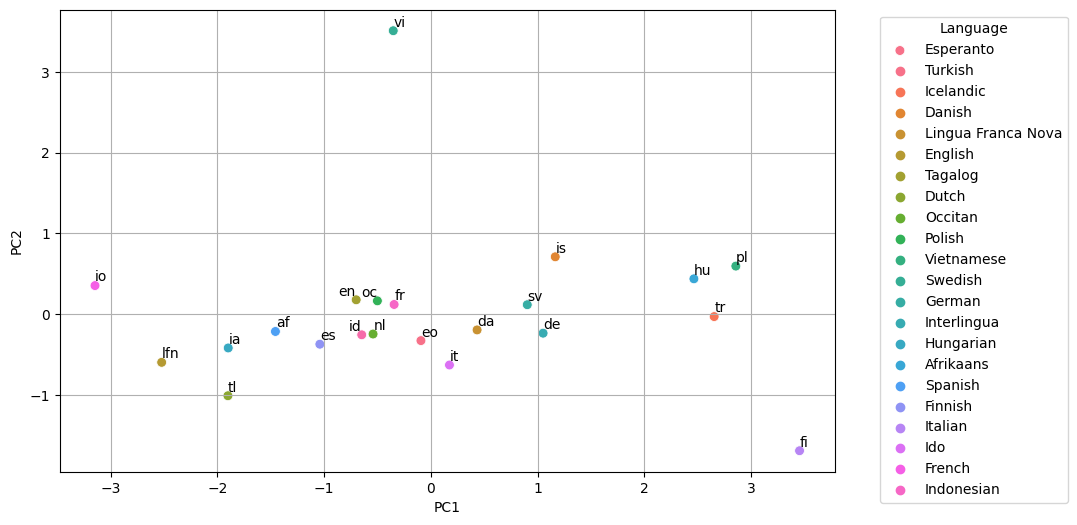
\includegraphics[width=1.0\textwidth]{pcaanalysis.png}
        \caption{Principal Component Analysis on TTR, MATTR, Word and Char Distribution Entropy}
        \label{fig:pcaanalysis}
\end{figure}

% Include graph of explained variance following https://www.jcchouinard.com/pca-explained-variance/

A script was used to increase readability of the text in the graph\footnote{https://github.com/Phlya/adjustText}.

\subsection{Results of One-Class SVM}
\label{ssec:oneclasssvmresults}

\subsection{Results of Decision Tree}
\label{ssec:decisiontreeresults}

\begin{figure}
  \centering
        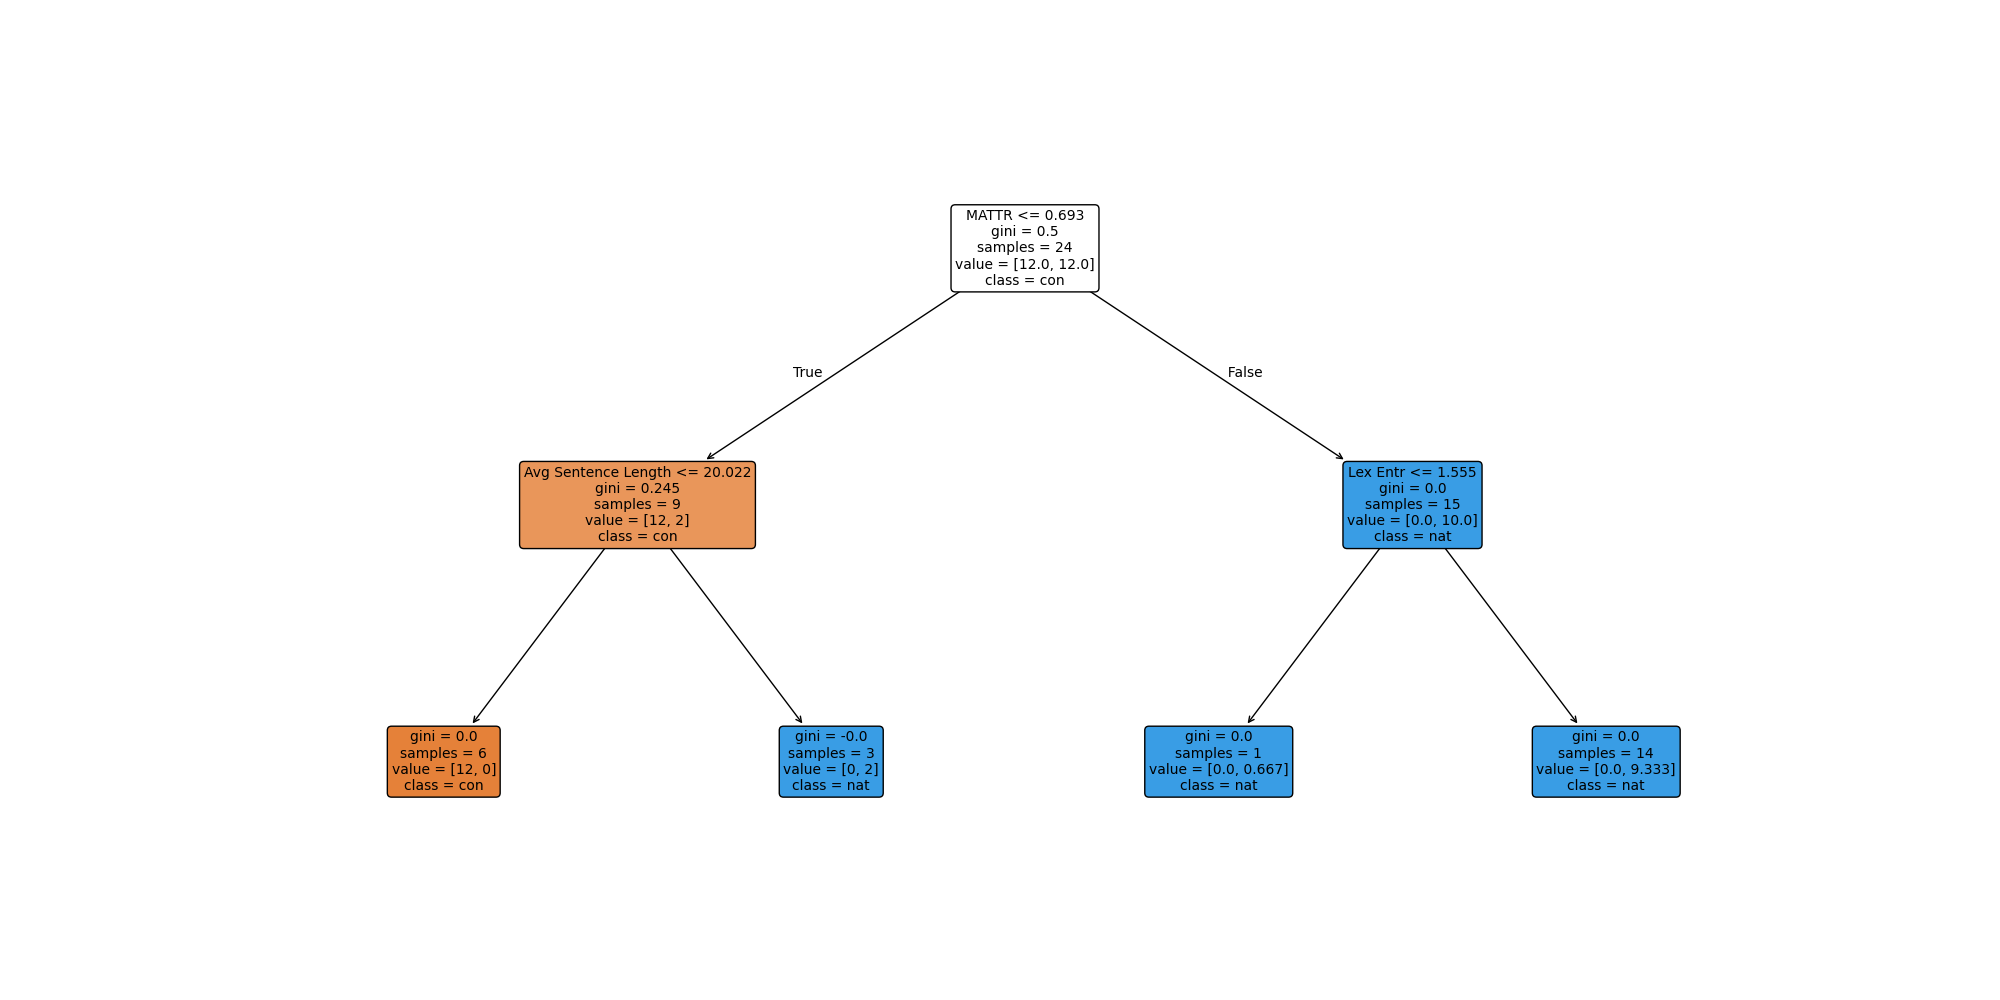
\includegraphics[width=1.0\textwidth]{decisiontree.png}
        \caption{Decision Tree Classifier}
        \label{fig:decisiontree}
\end{figure}

\subsection{Results of Random Forest}
\label{ssec:randomforestresults}

\newpage
\section{Discussion}
\label{sec:discussion}

% Mention expectations (e.g. the conlangs coming from European languages, so the models might confuse these with the natural languages when classifying the two) and how they compare to the results
% Come back to the question/topic of linguistic universals, how do these results fit into the debate?
% Discuss problems with morphological complexity analysis: lack of gold standard corpus to evaluate models' segmentations, etc

\newpage
\section{Conclusion}
\label{sec:conclusion}

\subsection{Future Work}
\label{ssec:futurework}

The research presented in this thesis is far from encompassing all there is to the topic of defining language, and distinguishing between constructed and natural language. At present, this is an area of research with ample room for potential development. 

Limiting factors: number of languages and which languages/language families, lack of real parallel corpora, problems associated with low-resource languages, relatively narrow scope of experimentation,

\newpage
\section{Acknowledgments}
\label{sec:acknowledgments}
I would like to thank ....

\newpage
\printbibliography

\newpage
\section{Appendices}
\label{sec:appendices}

Here I...

% Include number of symbols in the alphabet for each language? (Gomez 2014, Table 1)
\begin{table}[h!]
  \centering
  \renewcommand{\arraystretch}{1.5}
  \begin{tabular} {|p{3cm}|p{3cm}|p{3.5cm}|}
  \hline
  \textbf{Language} & \textbf{Number of Words} & \textbf{Number of sentences} \\
  \hline
  Icelandic & 629995 & 41847 \\
  German & 629987 & 37261 \\
  Polish & 629997 & 42138 \\
  Ido & 629990 & 43496 \\
  Afrikaans & 629994 & 30737 \\
  Kotava & 617400 & 48145 \\
  Hungarian & 629946 & 39916 \\
  Lingua Franca Nova & 628683 & 32188 \\
  Danish & 629999 & 38260 \\
  Spanish & 629978 & 24886 \\
  Interlingua & 629996 & 32229 \\
  French & 629983 & 27248 \\
  Occitan & 629998 & 33762 \\
  Esperanto & 629994 & 33317 \\
  Dutch & 629997 & 34627 \\
  Turkish & 629995 & 43573 \\
  English & 629958 & 29574 \\
  Tagalog & 629989 & 29855 \\
  Swedish & 629998 & 36370 \\
  Vietnamese & 629958 & 21115 \\
  Italian & 629987 & 24487 \\
  Volapük & 629999 & 55920 \\
  Indonesian & 629997 & 34683 \\
  Finnish & 629994 & 52637 \\
  \hline
  \end{tabular}
\caption{Lengths of each language's text after pre-processing.}
\label{tbl:preprocessedtexts}
\end{table}

% Include tables of all the hyperparameters of the two RNNs and two classifier models

% Include the regular expressions used in the pre-processing

\end{document}